\documentclass[12pt]{article}

\usepackage{apacite}
\usepackage[longnamesfirst]{natbib}
\usepackage{geometry} %for setting up margins
\usepackage{url} %this package lets a url appear in the bibliography
\usepackage[english]{babel}
\usepackage[autostyle, english = american]{csquotes}
\MakeOuterQuote{"}  % the previous lines make it so that the quotation marks all appear the right way around 

\usepackage{tabto}
%\usepackage{listings} %for inserting R scripts
%\usepackage{verbatimbox}

\usepackage{fancyvrb} %centre verbatim box

%for the figure stuff
\usepackage{subfig}
\usepackage{wrapfig}
%\usepackage{subfigure}
%\usepackage{subcaption}
\usepackage[justification=centering]{caption}
\usepackage[bottom]{footmisc}
% to set up the figures to be apa
%\captionsetup[figure]{labelsep=period,labelfont=it,justification=justified,singlelinecheck=false,font=doublespacing}
% add in font=doublespacing

\usepackage{fancyhdr} %Just used to make nice headers and footers 


\pagestyle{fancy}
\fancyhf{}
\fancyhead[LE,RO]{Penguins are cooler than you}
\fancyfoot[LE,LO]{Page \thepage}

\renewcommand{\headrulewidth}{2pt}
\renewcommand{\footrulewidth}{1pt}

\usepackage{graphicx}


\usepackage[normalem]{ulem} %this adds the \uline{} function which stops underlined titles from running off the page 
\usepackage{hyperref} % This package makes it so that your citations become hyperlinks to the web url provided or to the reference section... That's really cool [colorlinks=true,linkcolor=blue,citecolor=blue]

\geometry{a4paper, total={170mm,257mm}, left=20mm, top=20mm}
\usepackage{setspace}
\linespread{1.5} %says there's a problem but it seems to work for line spacing




\begin{document}

\begin{titlepage}
	\centering
	{\huge\bfseries Penguins are cool\par}
	\vspace{1cm}
	Warren \textsc{James}, \par
	Dr.~Josephine \textsc{Reuther}, \par
	Ellen \textsc{Angus}, \par
	Dr.~Amelia \textsc{Hunt},\par
	and\par
	Dr.~Alasdair \textsc{Clarke}
	\vfill
\end{titlepage}	


\newpage

%% ABSTRACT
\begin{center}
	\section*{Abstract}
\end{center}

\begingroup\singlespacing
\newpage
\tableofcontents
\newpage
\endgroup

%% Itroduction
\section*{Introduction}
\addcontentsline{toc}{section}{Introduction}
\paragraph{} Everyday we make use of our visual system in order to solve many problems. Whether these are to aid us in avoiding obstacles, or to find an item of importance, the ability to direct our attention proves invaluable. However, the extent to which we make these decisions in an optimal manner is subject to debate. 

\paragraph{} \cite{najemnik2005optimal} argue that human performance in a visual search task is predicted by that of a model ideal observer. This model aimed to reduce uncertainty as to the location of a target item by deploying fixations to locations likely to contain the target and reduce the overall uncertainty of the search space. To do this, the model accounted for the loss of accuity for space further from the central fixation and using this information to reduce the amount of uncertainty to an appropriate extent. In accounting for visual acuity, the model would be less likely to revisit locations that were already inspected to an appropriate extent. 

\paragraph{} This would suggest that we make decisions about where to fixate based on underlying scene statistics and account for our own limitations. However, this would seem to be a fairly resource intense process, which begs the question as to whether this would be an appropriate solution to the problem. With this in mind, \cite{clarke2016stocha} suggest that human performance in a visual search task can be characterised by a stochastic process. Instead of engaing in a resource intense calculation of where to fixate, they suggest that we make eye movements that we like to make in a more stochastic process. 

\paragraph{} As such, this leaves us with the question of whether we make principled fixations based on various factors, or whether we simply do what we like to do and fixate locations in a more random fashion. One way in which this question could be addressed is by simplay tasking people with making one sensible eye movement. If we fixate based on principle, then to complete a task such as this should prove to be trivial. 

\paragraph{} Much to the contrary it appears that people do in fact tend to struggle at making one sensible eye movement \citep{morvan2012human,clarke2015failure}. \cite{morvan2012human} developed a paradigm in which participants were to make a single eye movement in order to give themselves the best chance of success at detecting whether a target dot was positioned at the top or the bottom of a box \textbf{\textit{(point to figure when you have one?)}}. To do this, three boxes were presented on screen. One in the centre, with two boxes either side. Participants were told that they were to fixate one of these boxes and that the target would then appear in one of the two side boxes. Throughout the experiment, these two side boxes would appear at difference eccentricities, sometimes being placed very close to the centre box, and at other times they would be a large distance from the central box. When the boxes were all close together, the optimal strategy would be to fixate the central box and use one's peripheral vision to detect the target. However, as the boxes separated, performance would begin to decrease. In this case, participants engaging in the optimal strategy would switch to focussing one of the two side boxes as this would then give them the best chance of success. 

\paragraph{} The results of their experiment clearly demonstrated that people failed to perform this task in an optimal fashion. These results were further supported by \cite{clarke2015failure} who replicated this study with the addition of including other versions of the task that were not specific to eye movements. This would suggest that this failure is not constrained to optimal search, but more a general failure to maximise the chance of success. 

% really not sure this paragraph is that necessary? 
% potentially could be though...
% Too long, needs to be reduced... maybe the paradigm doesn't need to be explained as much?
\paragraph{} This same sentiment was demonstrated by \cite{Hudson2007probmove}. In their study, participants were tasked with reaching for a target displayed on screen within a time limit. However, they were to begin their reaching motion before they knew exactly where the target would be. Instead, participants were shown a display of points that could be the target. The display consisted of thin bars made up of many small squares. At the begining of a trial, some of these squares would turn white indicating they were potential targets. The distribution of these squares cold be altered so that they were evenly spread across the bars on screen, or they could be concentrated in one are such as the centre of the display. Participants were then to reach towards the screen and, after crossing an invisible threshold, the target would be made clear by leaving only one square still illuminated. What they found was that when the target was most likely to appear to one side, participants would still begin their reach towards a more central point. This would suggest that participants were opting for a strategy that allowed for a small chance of success at locations that were unlikely at the expense of overall success. 

\paragraph{} Behviour such as this is prevalent in many other tasks. \cite{KahnemanChoicesValuseFrames} and \cite{Gigerenzer2011} both discuss many ways in which people demonstrate sub-optimal behaviours and some potential explanations for the observed patterns. One potential line of inquiry may be that of motivation. In \cite{clarke2015failure} participants were offered little in the way of reward for being successful other than the value placed on success by each participant. It is possible that participants simply had not real motivation to succeed. There are studies suggesting that by adding a financial incentive participants begin to make use of more optimal strategies \citep{Goodnow1955,phillips1966conservatism}. By adding a clear motivation for success in the form of a financial gain for success, participants moved from employing strategies that attempted to be successful for all outcomes and began to focus more on those that were more likely.
% This is worded horribly... needs to be thought through... 

\paragraph{} However, this did not seem to encourage participants to perform more optimally in \cite{morvan2012human}, which may be due to this effect being more nuanced than simply giving people money for being successful \citep{Camerer1999}. As such, this does not rule out that participants performed poorly due to a lack of motivation. 

% talk about gamification a bit here 
\paragraph{} Even with this added financial incentive, the goals of a participant may still be maligned with the desires of the experimenter. For example, even though in \cite{morvan2012human} participants were rewarded for success, they may have prioritised completing the task as quickly as possible rather than gaining the largest sum of money at the end of the experiment. \cite{miranda2014intrinsic} discuss the idea that by using a more gamelike design, it may be possible to encourage participants to prioritise success rather than speed of completion. % need to expand this somewhat...

\paragraph{} In the present study, we attempted to motivate participants to want to succeed gamifying the problem. In doing so, we were able to examine whether participants would begin to make more optimal decisions when being successful was clearly stated as being the goal of the task. 

\section*{Methods}
\addcontentsline{toc}{section}{Methods}

\subsection*{Participants}
\addcontentsline{toc}{subsection}{Participants}
\paragraph{} Participants were recruited via word of mouth at the University of Aberdeen. In total, 18 participants took part in the experiment (13 female) with an age range of 20-23 (mean of 20). 

\subsection*{Procedure}
\addcontentsline{toc}{subsection}{Procedure}
\paragraph{} The experiment took part over two sessions. The first session was to measure each participant's visual acuity in order to tailor the second session to each individual. The first session lasted approximately 30 minutes. In the second session, participants carried out the actual decision task, which lasted between 40 and 50 minutes. 

\paragraph{} Both sessions made use of and Eyelink 1000 (version 4.594) (SR Research ltd, Mississauga, Ontario, Canada) which recorded eye position at 1000 Hz. Participants were sat $\approx45cm$ from the screen, which was maintained throughout the experiment by use of an adjustable chin rest. \textit{Was this experiment on the OLED?}. The experiment was programmed and run in Matlab 7.9.0 (R2009b) with Psychtoolbox \citep{pelli1997videotoolbox} and EyelinkToolbox functions \citep{cornelissen2002eyelink}. Prior to starting each session, a 5-point calibration was carried out. Participants were recalibrated prior to starting a new block. Additionally, they were also recalibrated if they had failed to fixate appropriately 10 times since the last calibration, or if there were 5 errors in a row.

\subsubsection*{Session 1}
\paragraph{} In the first session, participants were presented with a fixation cross with two boxes placed either side \textit{\textbf{get fig}}. They were told that their task was to identify whether a small dot \textit{\textbf{get size of this dot}} had appeared in the top or the bottom half of one of the boxes (each $\approx1^{\circ}$). It did not matter which box it had appeared in, they were simply to report whether it was up or down by pressing the "up" or "down" arrow, respectively, on the keyboard. The dot had an equal chance of appearing in either box and in either position. To commence each trial, participants had to press the space bar whilst fixating the central cross. After maintaining fixation for 700ms, the target dot would appear in one of the two boxes, at random, and was displayed for 700ms (\textit{\textbf{Need to double check all this}}). If participants broke fixation during any stage of this process, the screen would turn red for 700ms to indicate that they had broken fixation. 

\paragraph{} The boxes were presented at varying separations from the central fixation cross ($2.7^{\circ}$, $3.9^{\circ}$, $5.2^{\circ}$, $6.8^{\circ}$, $8.4^{\circ}$, $10.1^{\circ}$, $11.4^{\circ}$, $12.5^{\circ}$). There were 4 blocks in total, with each different separation being presenter 12 times in a pseudo-random order. This meant participants completed 4 blocks of 96 trials. Data from this session was then used to work out the point at which participants were 75\% accurate in detecting the target. This value was then used in the second session to tailor the experiment for each individual.

\subsubsection*{Session 2}  
\paragraph{} For the second session, participants were introduced to "\textit{Pugadoo}". They were told that there task was to help Pugado collect as many fish as possible. In order to do this, they would be choosing a box to fixate in order to detect whether the target dot was in the upper or lower half of one of the two side boxes (\textit{\textbf{Get fig}}). On each trial, participants would see Pugadoo and have to fixate the star on their stomach to start the trial. They would then press the space bar and three boxes would appear. Participants were told they could fixate any one of the three boxes but that the target would only ever appear in one of the two side boxes at random. These boxes were placed at various distances from the centrally presented box. These distances were defined in relation to the switch point that was calculated based on their performance in the first session. Seven were defined as the switch point in the following way; switch point $-3^{\circ}$, $-2^{\circ}$, $-1^{\circ}$, $0^{\circ}$, $+1^{\circ}$, $+2^{\circ}$, $+3^{\circ}$. A further two distances were added so as to be constants across all participants ($8^{\circ}$ and $18^{\circ}$). 

\paragraph{} For every trial that the participants correctly identified the position of the target dot, the background would turn green and the bar in the top left corner would fill by one tick. After having filled the bar to the top, Pugadoo would be rewarded with a fish and the bar would return to being halfway filled. If the participant was incorrect, the background would turn red and the bar would be emptied by one tick on the bar. If the bar was fully depleted, a fish would be taken away from the total. This allowed participants to monitor their performance while completing the task. 

\section*{Results}
\addcontentsline{toc}{section}{Results}
\paragraph{} All analysis was carried out in R version 3.4.3 \citep{R} using Rstan \citep{Rstan,Stan}. Additional data was retrieved from \url{https://osf.io/t6c5q/} in order to compare the current study's data to a group without the presence of a clear goal, but who otherwise carried out the same task. The full methods and analysis of this comparison data can be found by following the link provided. 

\paragraph{} For the purposes of this study, the first four blocks completed by participants in this comparison set were used. In the first four blocks of this other study, particiapnts either carried out the standard task as described in \cite{clarke2015failure}, or they were effectively instructed as to where they should fixate on each trial in order to achieve the optimal accuracy (henceforth referred to as the "\textit{control}", and the "\textit{optimal}" group respectively).

\subsection*{Fixation Proportions}
\paragraph{} On each trial, participants were given three possible locations to fixate. Fixations were coded as being either a central fixation (i.e., they fixated the centre box), or as a side fixation (i.e., they fixated one of the side boxes). A proportion was then calculated for how often the participant fixated one of the side boxes within each of the distances mentioned in the methods section. 

\paragraph{} From an intial inspection of Figure \ref{fig:Position_raw}, participants in the motivated group do not appear to be doing anything different to those in the Control group. They certainly do not look as though they have been instructed as to where to look if one compares their results to the Optimal group. 

\paragraph{} \textit{I do have model results for this... but I imagine this can be added to the supplementary material? Also, it's pretty uniformative as to what's happening and doesn't add more to what can already be seen in the figure anyway}

\begin{figure}[ht!]
	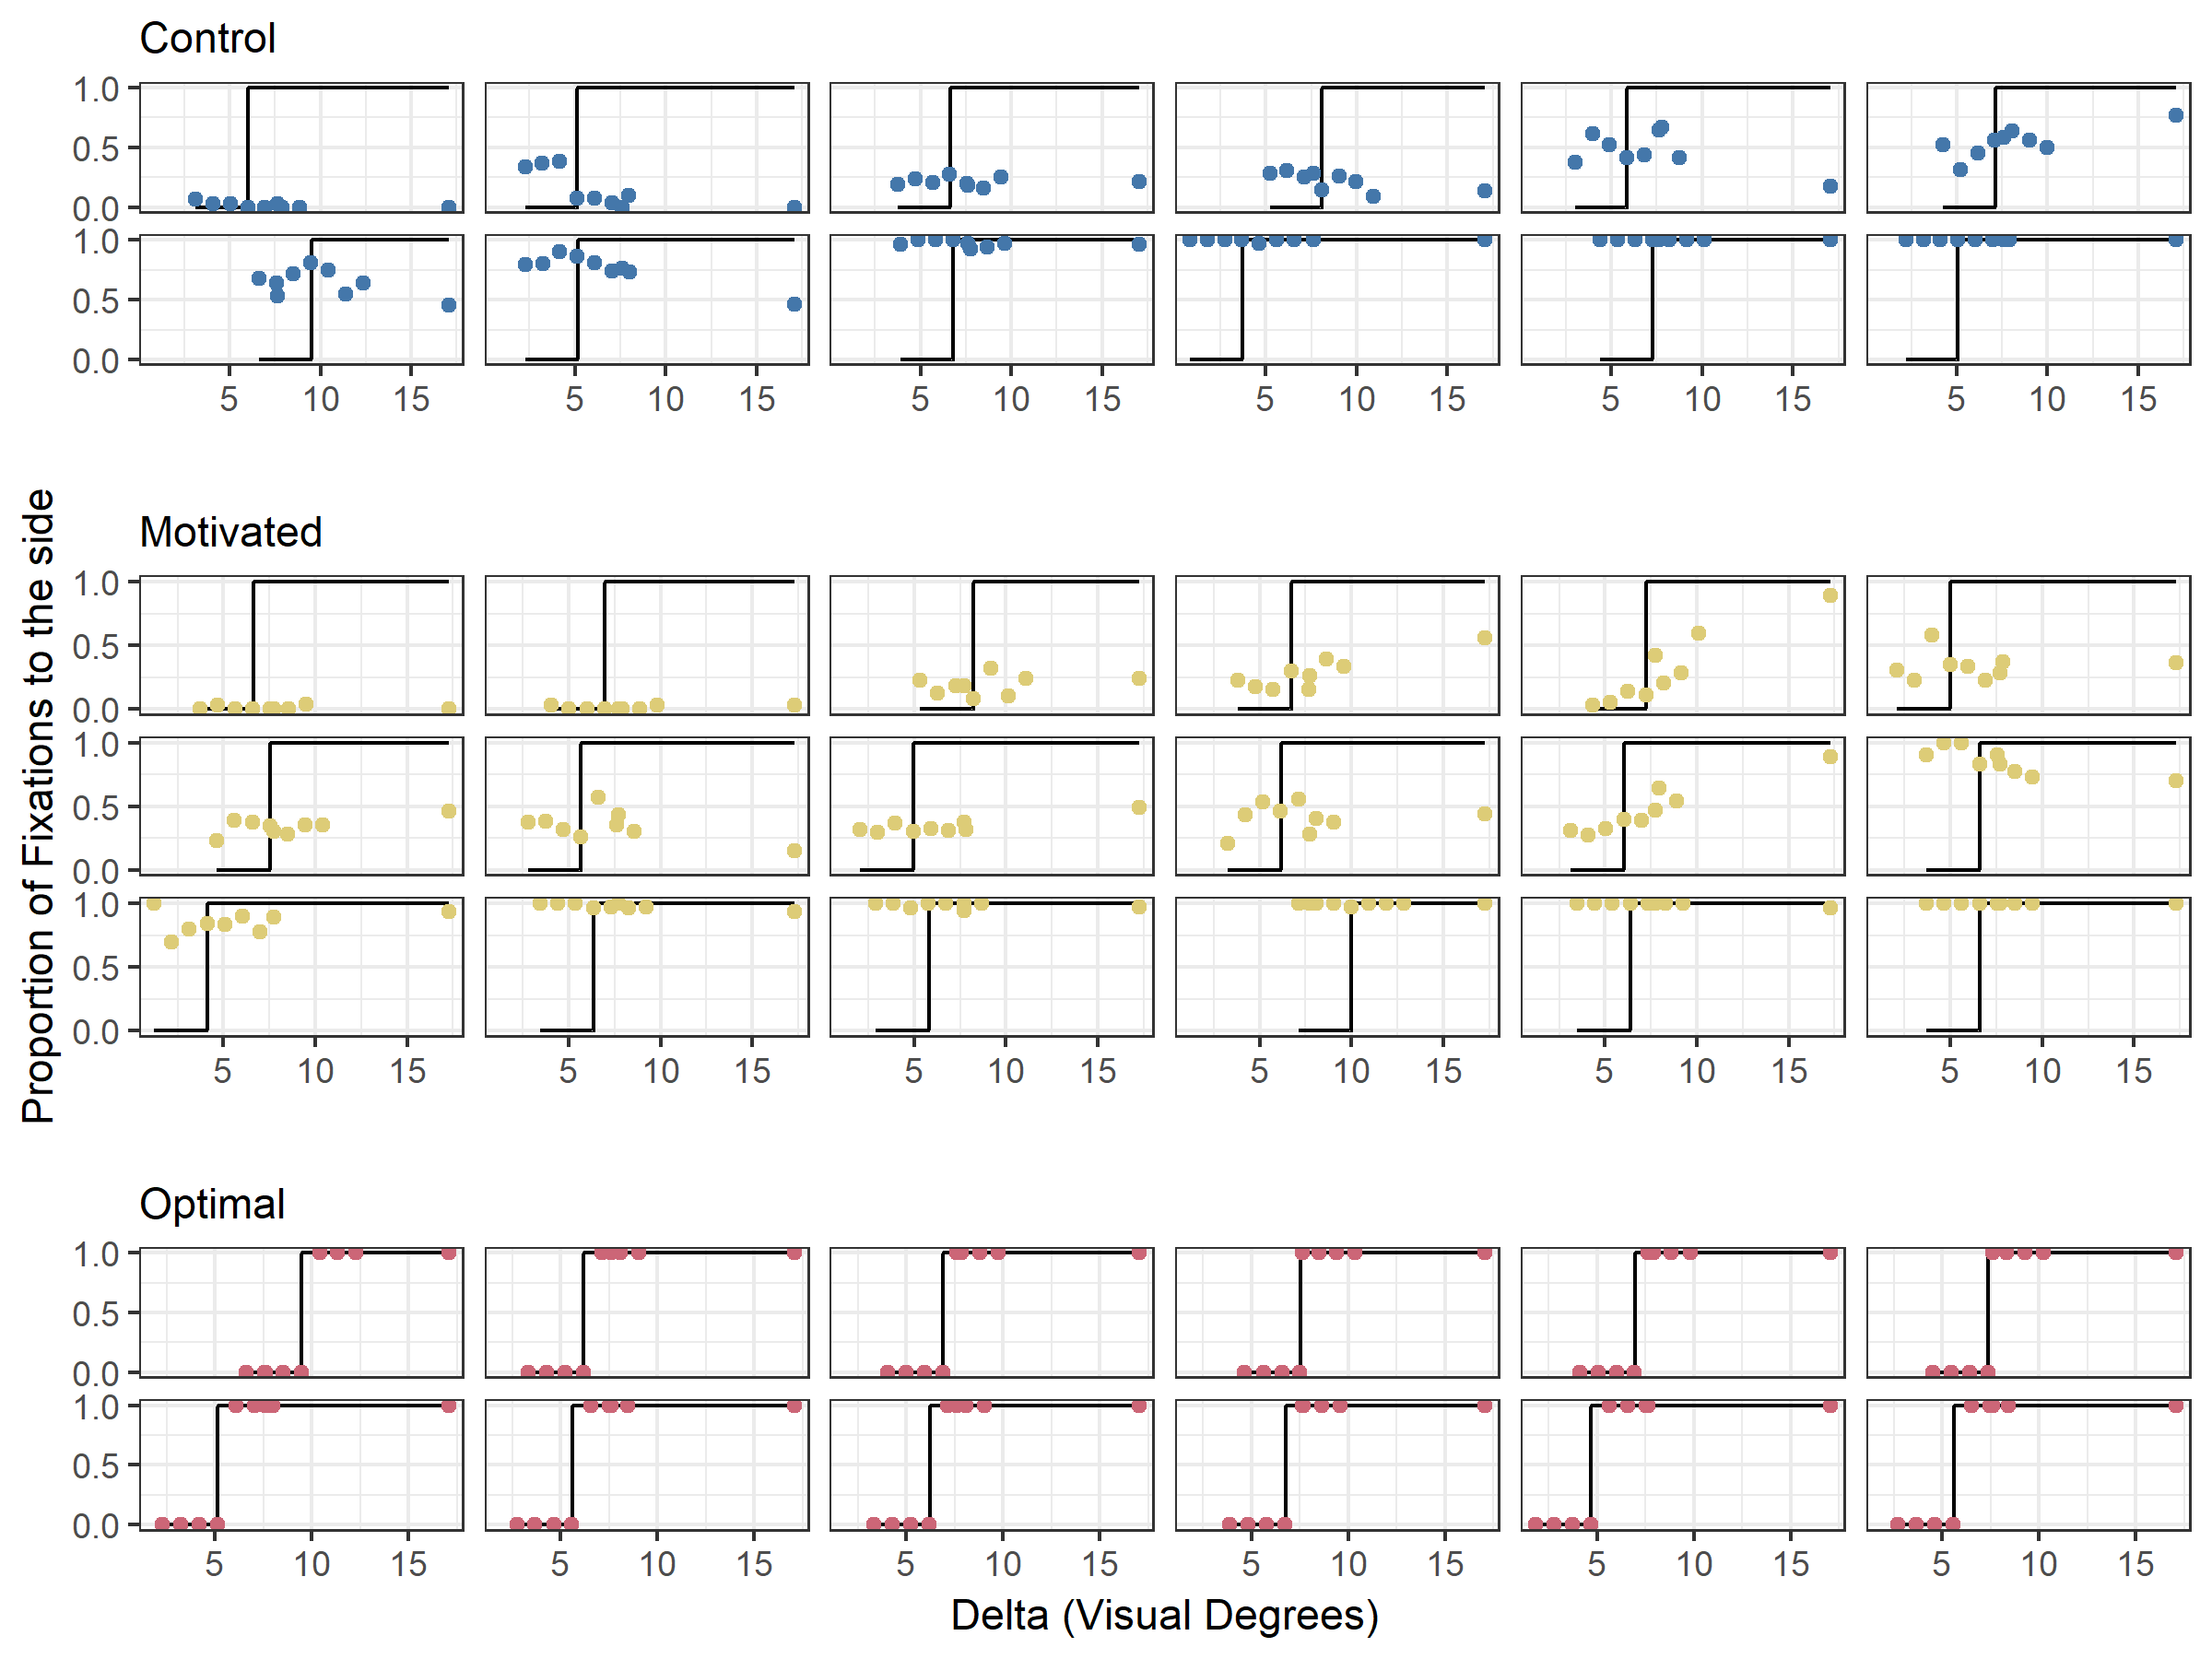
\includegraphics[scale=0.7]{../Figures/Part_2_all_groups.png}
	\centering
	\captionsetup{justification=centering}
	\caption{Plot of proportion of fixations to the side box (y-axis) with increasing Delta (x-axis). The bottom set of plots (in red) demonstrate what behaviour would look like if participants had employed an optimal fixation strategy}
	\label{fig:Position_raw}
\end{figure}

\subsection*{Rate of Success} 
\paragraph{} Initial analysis for rate of success examined overall accuracy for each pariticipant. To do this, an average was calculated for each participant which was then modelled using a Bayesian Regression Model with a Beta family. All priors were left as uniform and therefore uniformative. Rate of success was modelled using group as a predicor variable. Delta was not investigated as we are first and foremost interested in the participant's overall rate of success. 

\paragraph{} \textit{Should the analysis that included Delta be presented in the supplementary material? Pretty sure it does help with the model fit, but it's not entirely necessary for the conclusions of this paper?}

\begin{figure}[ht!]
	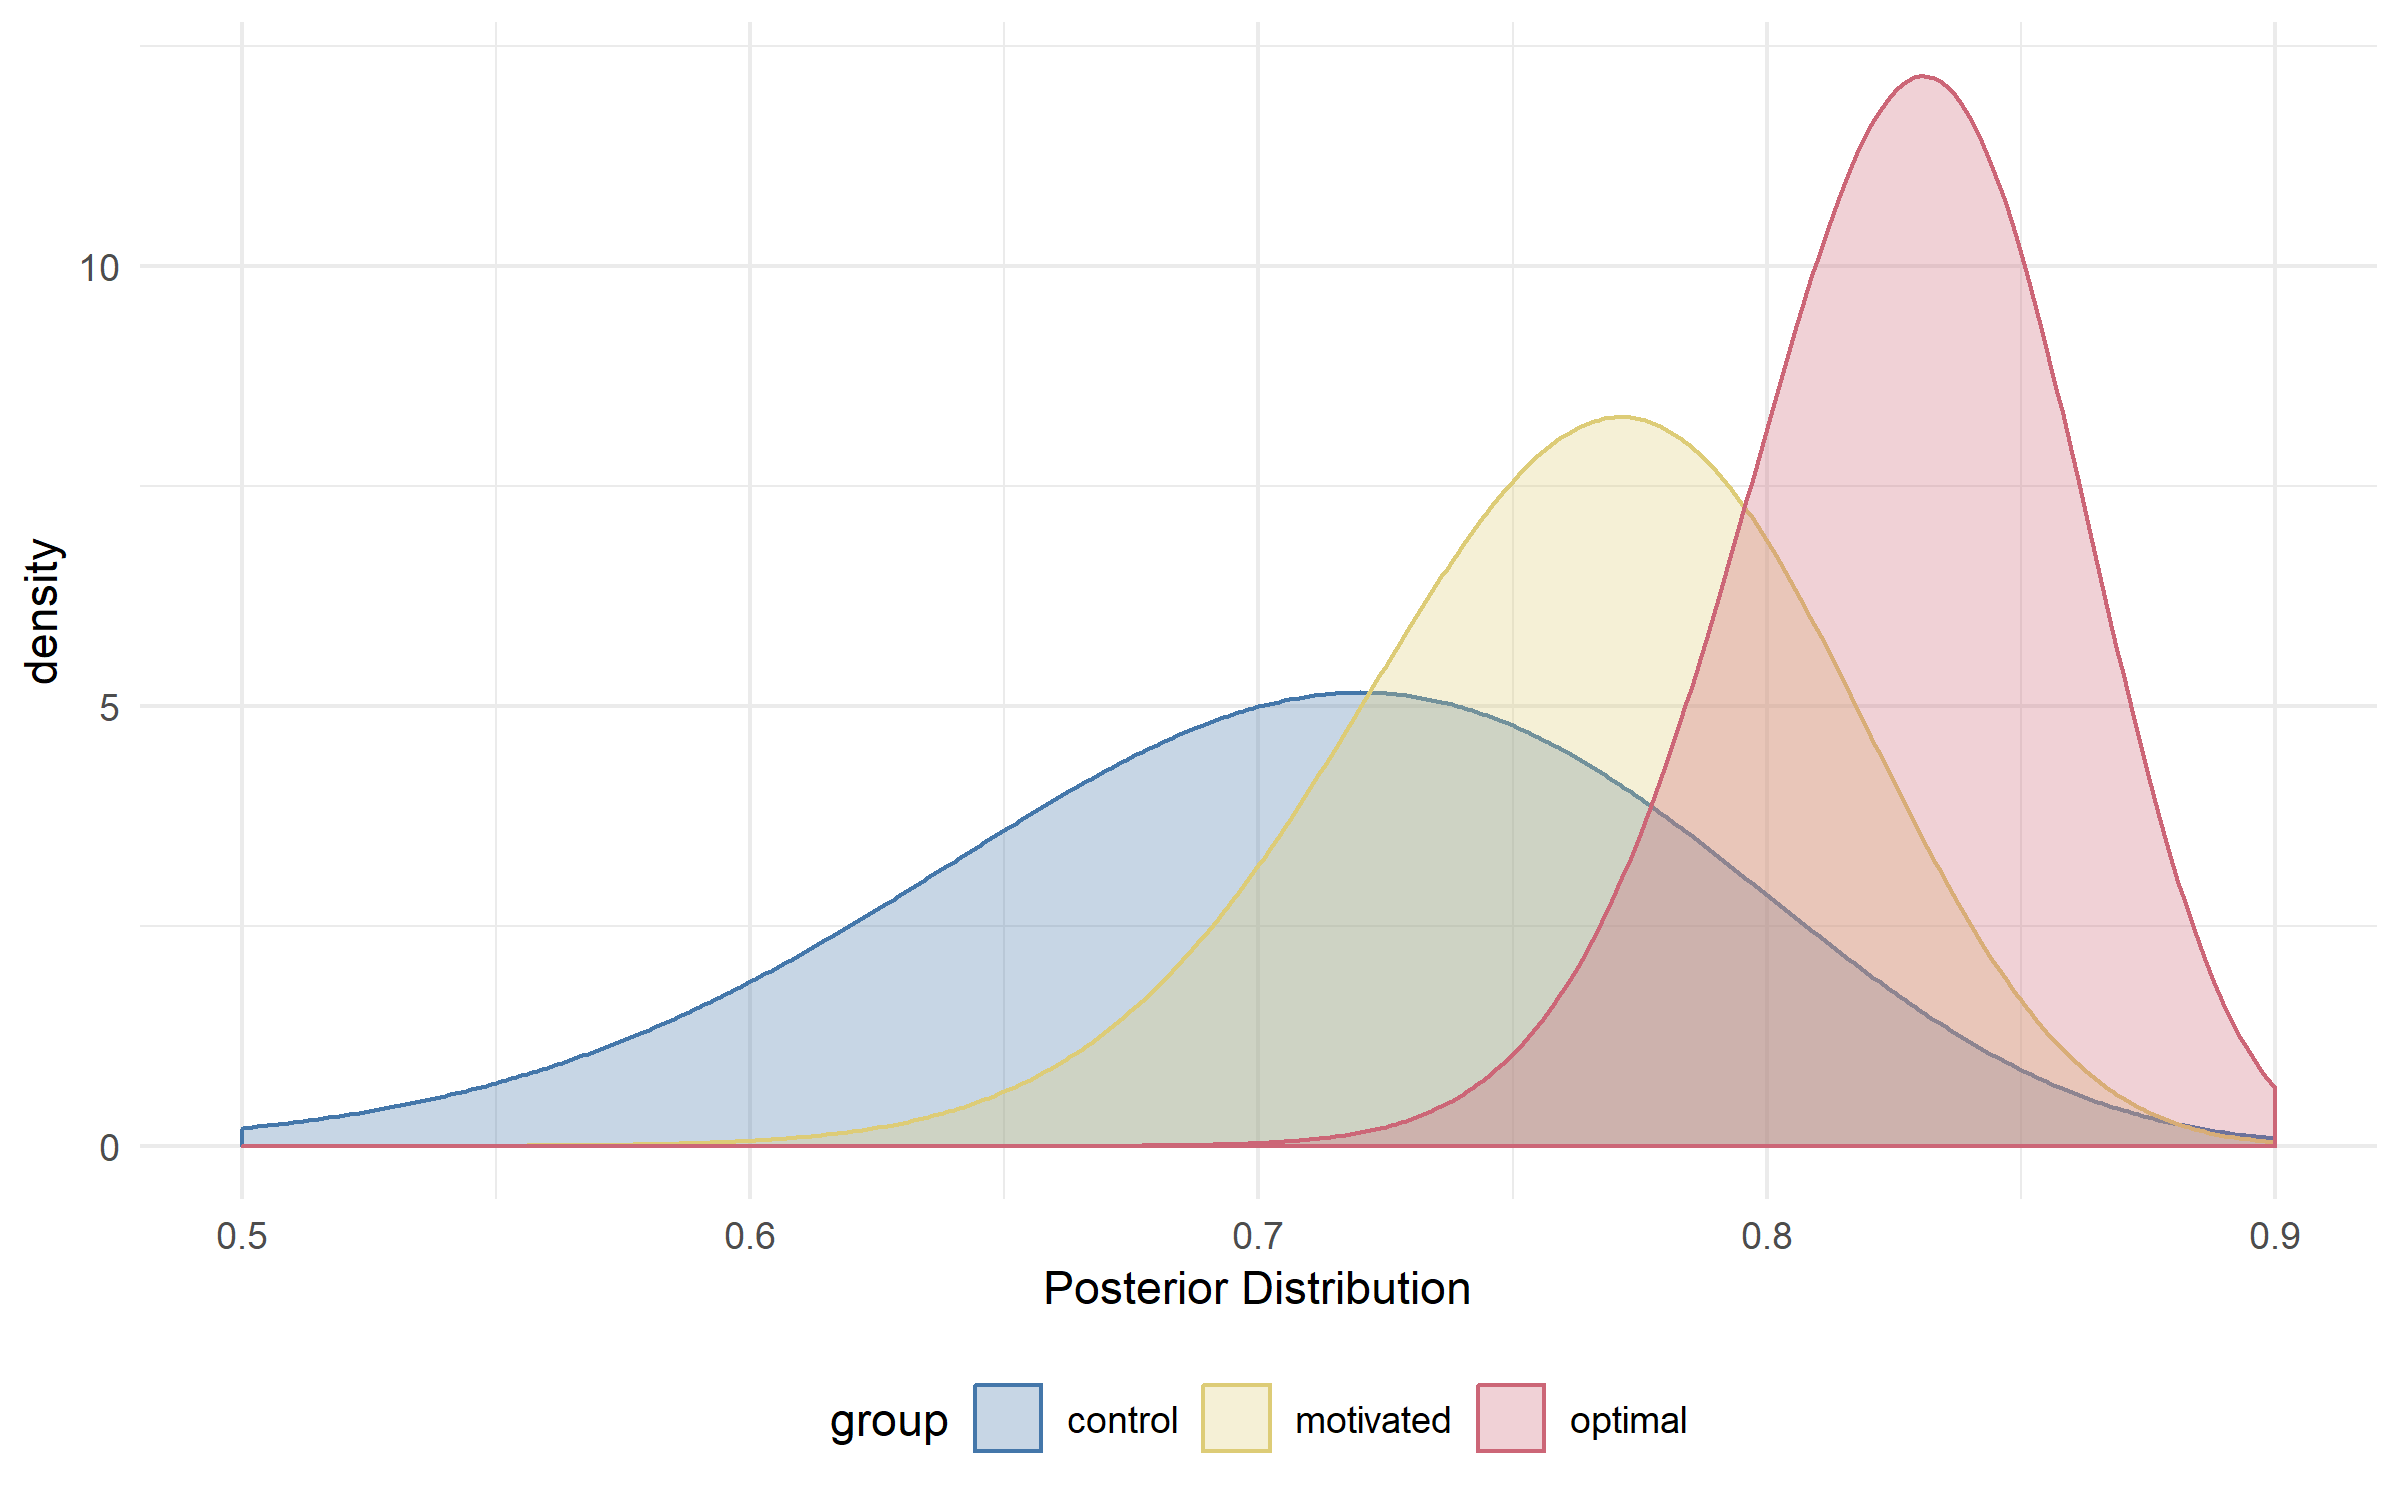
\includegraphics[scale=1]{../Figures/Model_stan_rawacc.png}
	\centering
	\captionsetup{justification=centering}
	\caption{Posterior predictions for rate of success.}
	\label{fig:Model_raw_acc}
\end{figure}

\paragraph{} In Figure \ref{fig:Model_raw_acc}, it can bee seen that that the Motivated group were generally more successful than the Control group. The Control group had a predicted mean rate of success of $0.708$ with a 95\% HPDI of $|0.661, 0.747|$, and the Motivated group had a mean of $0.764$ with a 95\% HPDI of $|0.74, 0.789|$. However they did not reach the same level of success as the optimal group which had a mean success rate of $0.825$ with a 95\% HPDI of $|0.805, 0.844|$. 

\paragraph{} This result seems somewhat surprising given the fixation proportions that can be observed in Figure \ref{fig:Position_raw}. As such, additional analyses were carried out.

\subsection*{Expected Rate of Success}
\paragraph{} In order to make a fairer comparison of the groups, each participant's expected success rate was calculated given the fixations choices they had made on each trial. For example, if the boxes were far apart and the participant had fixated one of the side boxes on that trial, they would have a $\approx$100\% chance of success at the fixated box (b$_f$) and $\approx$50\% chance of success at the non-fixated box (b$_{nf}$) as this would be imperceptable but they would have a 50\% ($c$) chance due to the nature of the task. Each of these boxes would be equally likely to contain the target and so the expected chance of success on a trial like this would be 75\% which is given by calculating $(b_f + b_{nf})\times c$. This was calculated for each participant, on each trial. This was then averaged for each participant to give an average expected accuracy. 

\begin{figure}[ht!]
	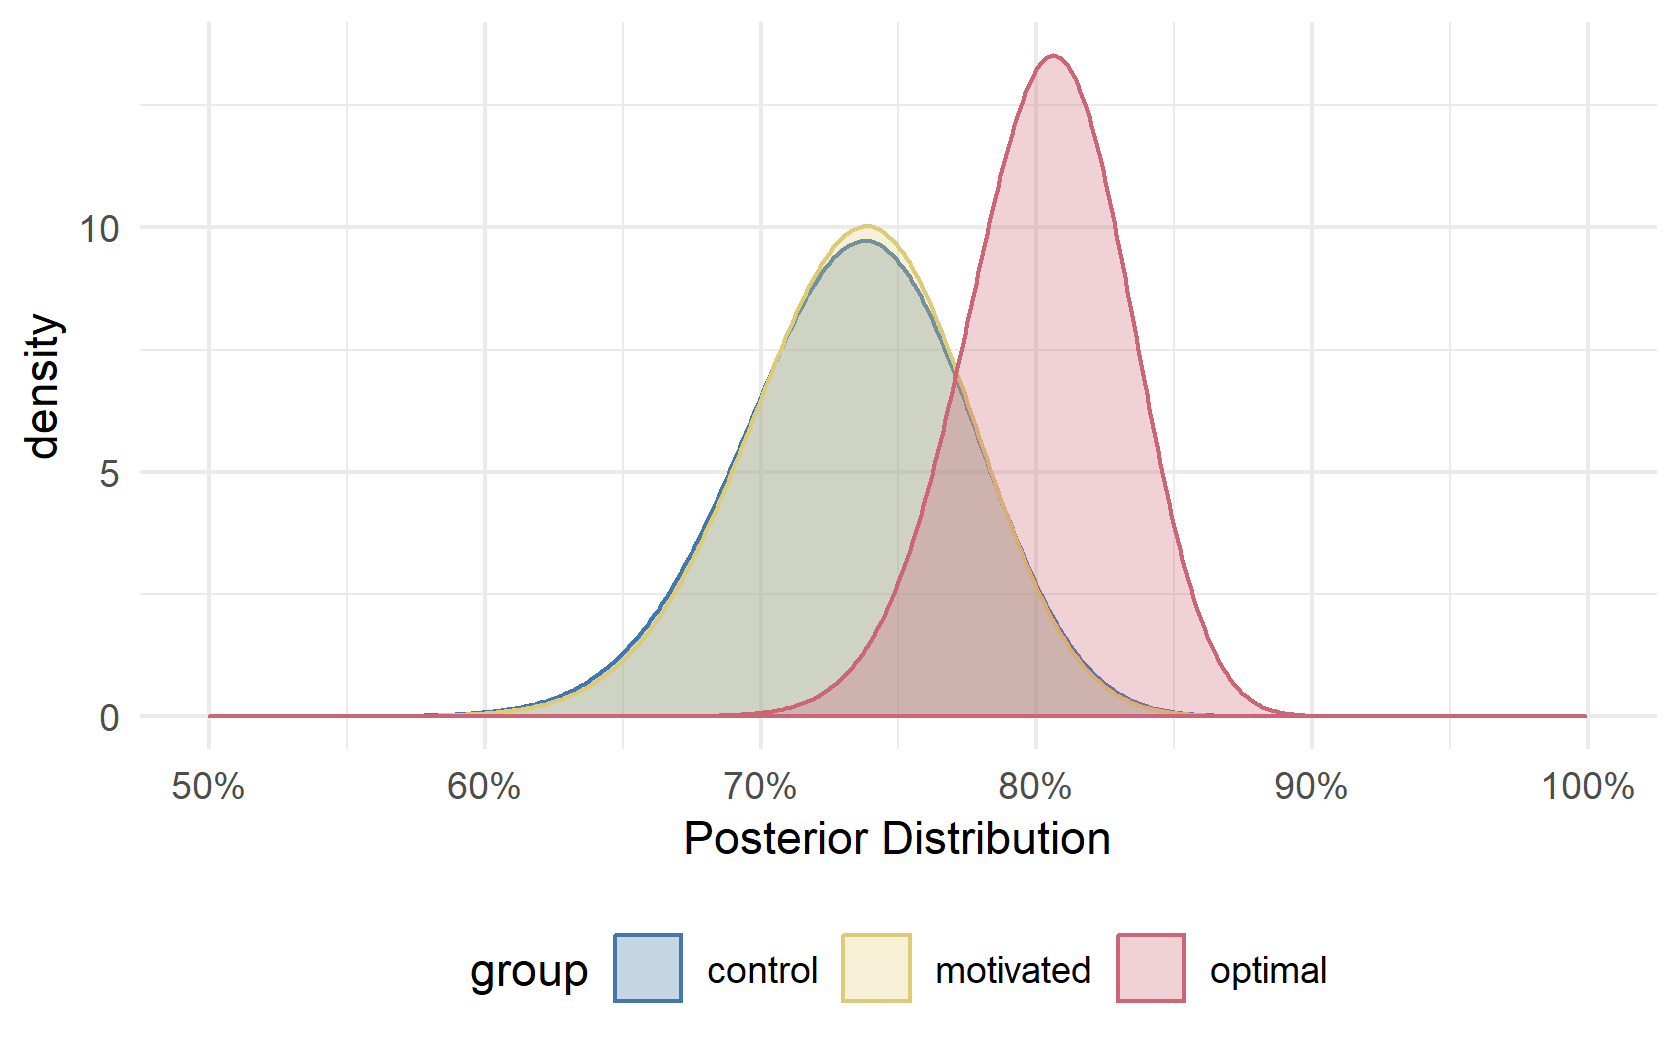
\includegraphics[scale=1]{../Figures/Model_stan_expacc.png}
	\centering
	\captionsetup{justification=centering}
	\caption{Posterior Predictions for expected success rate.}
	\label{fig:Model_exp_acc}
\end{figure}

\paragraph{} After accounting for chance, the difference that was once observed when modelling participant's raw success rate (Figure \ref{fig:Model_raw_acc}) appeared to entirely dissapear. Inspecting Figure \ref{fig:Model_exp_acc} would demonstrate that participants in the Motivated (mean of $0.735$, 95\% HPDI of $|0.715, 0.754|$) and Control (mean of $0.732$, 95\% HPDI of $|0.706, 0.755|$) groups almost identical expected success rates as can be seen by the almost entirely overlapping posterior predictions. These results would suggest that the previously observed greater rate of success experienced by the Motivated group was not due to them making better, strategical decisions about where to fixate. Instead, this greater rate of success would appear to be due to something other than a more optimal strategy being utilised. 


\section*{Discussion}
\addcontentsline{toc}{section}{Discussion}

\paragraph{} In this experiment, we attempted to encourage the use of an optimal strategy by including a clear motivation for success. Upon examining Figure \ref{fig:Position_raw}, there would appear to be no difference in strategy between the \textit{Motivated} and \textit{Control} groups. This would suggest that having a clear motivation for success does not cause people to begin to use optimal strategies. This could be expected given the similarity in results of \cite{clarke2015failure} and \cite{morvan2012human} in which the former provided no incentive, and the latter rewarded participants with a monetary sum for each successful trial. The results from this experiment are broadly consistent with previous findings in that participants appear to be quite variable when approaching this task.
 
\paragraph{} An interesting finding is present when looking at the particiapnts' rate of success in each condition. As would be expected, the \textit{Optimal} group had the greatest average rate of success. However, despite very appearing very similar in their strategy, the \textit{Motivated} group appeared to have a much greater rate of success than the \textit{Control} group (Figure \ref{fig:Model_raw_acc}). To investigate this further, we calculated a predicted rate of success for each participant given their choices throughout the task. After accounting for each choice, this difference all but disappeared. As such, this increase in accuracy does not appear to have been due to a more optimal strategy use as the \textit{Motivated} group now appeared almost identical in their expected rate of success (Figure \ref{fig:Model_exp_acc}).

% Although when comparing the raw rate of success for participants (Figure \ref{fig:Model_raw_acc}), it would have appeared that participants in the motivation condition were generally more successful. However, after accounting for the decisions participants made, this difference reduced to virtually nothing (Figure \ref{fig:Model_exp_acc}). It would appear that by adding a motivation for success, participants did not improve their performance by making more optimal decisions and instead must have gained this increase in performance by other means. 

\paragraph{} This change in accuracy in the absence of an improved strategy could be explained by participants making a greater effort to be successful. Rather than employing a better strategy, it is possible that participants were instead merely expending more effort to detect the target. In an experiment by \cite{engelmann2007motivation}, they found that participants' sensitivity to detecting a small target increased when a greater monetary reward was associated with success. They suggest that this increase in performance could have been due to more effort being expended on behalf of the participants in order to detect the target, and therefore raise their rate of success. 

\paragraph{} In an experiment conducted by \cite{manohar2017distinct} found that participants did indeed expend more effort when their success was rewarded. They wanted to investigate whether the mere presence of reward would enhance effort, even when the earning the reward was not contingent on making a greater effort. In their task, particiapnts were instructed to fixate a central cue. They were then informed about how the reward for success would be determined on that trial. A target would then appear either to the left or right of the central fixation. Participants were told prior to each trial how the reward would be determined. There were four ways in which this happened; participants would receive the reward if their response time was in the top 50\% of response times, at random, a guaranteed amount, or a guarantee to not receive anything. To compare effort in this task, they measured the time taken to fixate the target. What they found was that participants were much quicker to fixate the target when rewards were contingent on performance and if there was a guarantee of receiving a reward, though the latter was to a lesser extent. 

\paragraph{} This demonstrates that even in a situation in which extra effort is not stricly necessary, the mere prospect of a reward can cause people to expend more effort in pursuit of the reward. As such, this could perhaps explain the results observed in the current study. Although participants did not make better decisions, they may have been working harder to be succesful in the task. 

\section*{Conclusion}
\addcontentsline{toc}{section}{Conclusion}

% Bibliography
\clearpage
\begingroup\onehalfspacing
\newpage
\addcontentsline{toc}{section}{References}
\bibliographystyle{apacite}
\bibliography{MD_bib}
\endgroup

\end{document}